% 来源：OEBPS/Text/Section0001_split_003.xhtml#sigil_toc_id_26

\BookChapter{16}
\section[第16章\q 你的计划是什么？]{第16章\\ 你的计划是什么？}

\begin{BookQuote}
如果你不知道要去哪里，那么你走哪一条路也无法抵达。

\hfill ——亨利·基辛格
\end{BookQuote}

祝贺，你走了很长一段路了！经历了通向财务自由的三大步。你已经做了你一生中最重要的财务决策。你已经成为一个投资者，承诺保持或者不断扩大你的收入自动储蓄比例，把这些钱自动地转到你的自由基金里。你已经开始建造让你自由的赚钱机器。你已经学会了如何保护自己，不受那些最大的投资营销谎言的欺骗，这些谎言早就想把你和你的钱分开了。最后一步是，你已经给你的梦想标出了价码。你知道需要多少年收入才能实现财务自由和财务独立。现在我们将会利用你学到的复利的力量，把这些金钱威力法则付诸实施。我们会一起努力给你和你的家庭创建一个规划，这是绝对可以实现的，而且在你的能力范围之内，不管你们的目标是什么层次的财务梦想——安全、活力、独立，这个计划都适用。

在我们开始之前，还有另外一件事需要做，即使你像大多数人一样痛恨谈论金钱。不过，没关系，没有其他人能看见这些数字，除非你决定给他们看，与他们分享。最重要的是你对自己要诚实。在这里就不要为了面子粉饰数字了，不要歪曲事实了，不要戴着玫瑰色透镜来看你的“数字”了。同样的原因，也不要强迫自己制订非常保守的计划，因为你觉得计划制订得高了，自己不可能实现。自己对自己要实话实说，承诺一定要实实在在地看清现实，自己现在的财务状况究竟是什么样子。只有实事求是，实话实说，才能让这个投资理财规划真正地起作用。

\subsection{你只能靠自己的双手来奋斗}

我有一个好朋友，最近和他从小玩到大的小伙伴相聚，以庆祝他们的50岁生日，聚会地点就在棕榈滩上我们住的房子旁边。他们一起上的幼儿园，住在一条街上，上同一所高中，都住在纽约长岛上的莱维特社区。他们的父亲或是上班族，或是自己开公司的老板，他们的母亲都是家庭主妇，他们的家庭收入都差不多。这些一辈子的好朋友，最打动我的是每个人后来的发展情况。在他们的青少年岁月中，他们彼此的发展是同步的，但是离开家乡上大学之后，这些年轻人开始分别向不同的方向发展，差别很大：

一个人去了华尔街发展，在一家大型金融机构工作。

一个人成了摄影师，在曼哈顿开了一家照相馆。

一个人在亚特兰大中部地区搞房地产开发。

一个人开了一家公司，进口高档葡萄酒和精酿啤酒。

一个人接受培训，成了工程师，在佛罗里达州南部做公务员。

当他们重新聚会的时候，他们互相讨论、交换意见。虽然收入和财富有相当大的差距，但他们都过得很开心——尽管开心的形式不同。他们个人的需要得到了满足。他们的希望和梦想很多也得到了满足。

我让这个朋友读了本书的初稿，他这次聚会时跟他的好哥们儿分享了我在书里讲的一些投资理财观念。那是他们喝了几瓶啤酒之后，谈话的主题就转到了钱上，他们开始问彼此一些问题，这些问题跟你在前一章回答的问题一模一样：你需要积攒多少钱才能达到财务安全？或者需要多少钱才够支撑你的退休生活？那个在华尔街工作的人，觉得至少需要积攒2000万美元，才能保持现在的生活方式，而不用再靠工作赚钱；那个曼哈顿的摄影师认为，自己需要有1000万美元才够；那个房地产开发商觉得，有500万美元就可以搞定了，主要是因为现在他的孩子就要大学毕业了，少了很大一笔学费开支；那个卖葡萄酒的商人再婚了，尽管又要再生一个小孩，但他觉得能够攒到200万美元的退休养老金就够用了；那个公务员，一直想方设法地靠着他微薄的工资生活，习惯量入为出，未来就指望着靠那份稳定的养老金来度过余生了，他认为只要他开始领公务员养老金，再加上领取社会保险养老金，他就可以衣食无忧地享受退休生活了。

这些人哪一个更接近于自己的目标？对于需要积攒多少钱才够退休养老，谁估计的数字比较准确？谁有正确的投资理财规划来帮助自己顺利地达到目的？当然，这个问题隐藏着陷阱。因为答案并不是由金钱来决定的。你要赢得“人生的比赛”，并不能只靠积累最多的金钱，或者积累最多的财富。人生的竞赛也不能靠抓住机会快速领先，轻松到达终点来获胜。

那么你怎样才能赢？你要赢，只能按照你自己的想法来生活——做到你能做到的最好的样子，做到你能做到的那么圆满，做到你能做到的那么长久。

你制订一个计划，它符合你的需要，对你有效，你一直坚持执行，这就是成功，简单又朴实。如果你正在和别人攀比，和别人竞争，但你用别人的观点来界定成功，这样做的话，你想要实现的是一个遥不可及的目标，那么你就会落后，就会很受挫。如果你正在追逐的是别人的目标，你就会输。其实，你的邻居和同事有多少钱，开的是什么样的车，如何度假，这些都不重要。这个计划只针对你自己，只有你自己，跟其他所有人都无关。

\begin{BookQuote}
你停止比赛的那一天，就是你赢得比赛的那一天。

\hfill ——鲍勃·马利
\end{BookQuote}

\subsection{有时领先优势只是错觉}

你看过奥运会上的田径比赛吗？你很容易看到，在赛道上，发令枪打响之前，那些选手在不同的跑道上，起跑位置明显有先有后，外道的选手起跑位置比里道的选手明显靠前，可是结果表明，这并没有给他们带来巨大的优势。事实上，我们用脑子一想就知道，所有的选手跑的距离是相等的，但是我们肉眼看起来好像差别很大，眼睛欺骗了大脑。所谓的起跑位置领先，其实是一种交错安排，因为在椭圆形赛道上，这样交错安排起跑位置，才能使每个选手跑的距离相等。在400米比赛中，相邻两个选手的起跑位置要相隔6米，才能做到奔跑距离都是相同的400米。

当然，每个人都知道，实际上，你不管是在外道的起跑位置，还是在内道的起跑位置，其实你都没有任何优势。你跑的距离都是一样长的。但是表面上的起跑优势可能会给你带来一个很大的心理优势。那个跑在外道的人会觉得自己有领先优势吗？这会不会提高他的自信心，或者带走他一小部分的动力？那个起跑位置“靠后”的人会觉得大家都不看好自己，这会不会反而刺激他跑得更快，以做补偿？

我们回到那5位聚会的朋友，从旁观的角度进行分析，你也许会觉得，那个公务员看起来起跑的位置最靠后，那个华尔街的金融企业高管的起跑位置最靠前，他可能会大幅领先，直达终点，但这只是感觉，而不是现实。没有人领先，也没有人落后。

这里没有人排在第一的位置，也没有人排在最后的位置，生活不是一场竞赛，人们经常用钱或者得到的东西多少来衡量他们现在所处的位置：谁有更好的房子，更酷的车；谁在度假胜地汉普顿斯有度假屋。但是真相是，我们并不能预测我们会活多长时间，或者我们年老后的身体健康状况。真相是我们从哪里开始并不重要，重要的是我们如何结束。看起来，好像这5个人都在向着正确的方向前进——每个人都是按照自己的想法、自己的时间安排前行，这是他们对自己的生活感到快乐满意的原因之一。用一点纪律，加一点远见，他们现在都在努力赢得比赛，他们开始时是同时起跑的，他们是同时上幼儿园的。

同样的事情也会发生在你身上。不管你站在哪里，和你的朋友、家人、同事、客户相比，起跑位置靠前还是靠后，这都不重要，重要的是你自己的人生旅程怎么走。你忍不住会和别人比，这是人之常情。人生的赛跑是一场马拉松，不是百米短跑。你唯一要做的事就是专注于前面要跑的路，向前看，找到自己的跑步节奏，一直向前跑。制订出一个规划。

\begin{BookQuote}
你应该努力超越的唯一一个人就是昨天的你。

\hfill ——无名氏
\end{BookQuote}

\subsection{你的规划}

你知道了，你唯一的竞争对手就是你自己，现在是时候做个规划，画出你投资理财的蓝图。好消息是，所有你需要做的事就是打开手机App，回答6个问题。用这个理财计算器，只用几秒钟，你就能制定出自己投资理财规划的1.0版本。

这6个问题包括两个方面：你现在在哪里，你要如何努力前行。你回答这些问题需要的几个数据，看看你平时的账单就能找到，有的一拍脑袋就想起来了。你也许需要做一点点功课，但这些数字大多数都唾手可得——一时找不到也没关系，先大致估计个数字也行，最重要的是让自己先干起来，保持冲劲，不能停。

有了这些数据，这个App就能为你度身打造一个投资理财规划。当然，有些参数必须由你本人来决定，比如，你预期你的收入会增长多少，你决定要储蓄多大比例的收入，你预期自己的投资收益率会有多高。你可以估计得保守，也可以激进——你也可以有些地方做保守估计，有些地方做激进估计，有些地方介于二者之间。用这个App的最大好处是，你只要设定好这些基本变量就行了，余下的大量工作它会自动完成。你制订了一份白纸黑字、实实在在的投资理财规划，这就是你的未来财务发展蓝图，这样，以后你做事心里就有谱了。

\subsection{选择你自己的冒险之路}

你下载的App里，有个理财计算器。这个计算器我用了30多年了，我在工作室和研讨会上都会用它。这个App既简单又灵活，而且帮助几百万人创建了投资理财规划，很实用。这个规划基于一系列谨慎保守的假设，不过你完全可以修改这些假设，你想怎么改就怎么改。你可以设置得更加保守，也可以更加激进，这完全由你来决定。所以你输入数字时不用多想，只要适合你，符合你的生活方式，符合你现在的实际情况，符合你未来的梦想就行。如果App做出来的规划你不喜欢，没关系，你可以调整你输入的数字，选择另外一条不同的路径通向财务自由。在后面，我们一起努力，让你学会走出特别的几步，加速你的计划实施，确保你能够成功。你制订出的第一个投资理财规划，就好像是你咬的第一口苹果。接下来，我们开始实施这个规划，并逐步改善，后面我会详细叙述……

在我们开始之前，有几件事你需要牢记在心。

其中较大的影响因素之一是我们的税率，人和人之间会有很大的不同。读本书的人来自全世界，与其把税率这个事情搞得非常复杂，不如搞得特别简单。不管你住在哪里，在后面的内容里，你都会学会如何运用这些工具，在你的国家得到最高的税收效率。不管在哪里，只要有可能，你就要运用有税收优惠的账户来积累你的财富。这样做，你的税后净收益率会更高。

你输入数据后，这个理财计算器会显示给你三种可能的情形，每个计划分别对应着不同的年收益率：4\%、5.5\%、7\%。这三份计划分别是：一份保守的规划，一份适中的规划，一份激进的规划。这些收益率都是税后的净收益率。有些人也许会觉得这些数字太保守或者太激进了，你都可以调整成你喜欢的数字。

我们提出这三个数据有什么依据呢？在高的那一端，根据嘉信理财公司的标准，激进的收益率是10\%。我们的App设定的激进的收益率是7\%，为什么会有3\%的差异？嘉信理财公司的研究表明，在过去40年里，即1972—2012年，美国股市的平均收益率是10\%，但是我们的App计算器假定你要交纳约30\%的税，那么这会让税后收益率只剩下7\%。美国长期投资的税率只有20\%，不是30\%——所以说我们的App在税率设定上比较激进。而且请记住，如果你做投资用的是一个可以税收递延的工具，比如401(k)账户、个人退休金账户、年金，你可以递延纳税。所以如果你的投资有10\%的收益率（就像嘉信理财公司所说的那样），你可以继续按照10\%的收益率进行复利计算——在最终卖出变现之前不用扣税。我们用更低的收益率假设：4\%、5.5\%、7\%，这样可以提供一个安全垫，为你做投资出现错误留出一些余地，或者预防未来收益率没有达到你所期望的那个激进水平。\footnote{\label{fn:pdf-16-1}我写本书的时候利率已经让政府压低相当长时间了。不过只要利率一上升，这个App就会马上更新利率。你任何时候都可以调整App的投资收益率水平设置，只要你觉得适合你的情况和真实投资目标就行。}

在低的那一端或者说保守的那一边，你看先锋公司，它用的是税后4\%的收益率。但是我们的看法有些不同，大多数美国人用钱来做投资的话，都是通过401(k)账户、个人退休金账户或者罗斯401(k)账户进行的。哪个是最好的选择？我们推荐你用一个罗斯账户（或者你们国家对应的免税账户），除非你真的可以确定你的税率将来会变得更低（祝你好运）。全世界所有国家的政府，特别是美国政府，总会提前花掉它们手里没有拿到的钱，那它们怎么来还这笔钱？手段就是提高税收。所以尽管没有人可以确定未来的税率是高还是低，我敢打赌未来的税率肯定会提高。使用罗斯账户，你的投资收益就不用纳税，收益100\%都是你的。比如，如果你得到了7\%的收益率，你可以把7\%的收益全部保留下来——你的投资增值不用扣一分钱的税。如果你得到了10\%的收益率，这10\%的盈利你可以全部留下。

正是因为这个原因，我们要用这种方式打造一个投资理财计算器。这样能给我们灵活性，用税后（净）收益率来思考投资收益。你设计的投资理财规划要用你认为的对于你的目标来说最合理的指标。

我们设计这个投资理财计算器的目的是让你快速感觉到，不同的选择会有不同的影响，这导致你实现财务梦想所需要的时间长短不同，不管你的梦想是财务安全，财务活力，还是财务独立。你制订出来一个你喜欢的基本规划之后，还可以进一步完善，输入更加精确的数字。我在前面说过，堡垒投资理财公司有一个技术平台，可以链接你所有的投资账户。这个平台会马上反馈给你这些投资过去的实际收益率是多少（大多数人对此根本一无所知）。它还会显示出，哪些年份业绩表现最好，哪些年份业绩表现最差，哪些年份发生了亏损。这个平台还会显示出你实际支付的费用是多少。这样你会知道，这些费用对你未来积累财富的实际影响有多大。你先在App上制订出一个基本的投资理财规划，再登录网站，查找你过去的历史收益率，让你的规划更加精确。

当然，在这个App中，你的那些数据和你的规划完全安全，不会丢失，而且不管你人在哪里，用什么设备，都可以随时获取信息。任何时候，你都可以改变你的收益率设置，改变你愿意储蓄的比例，你很快就能看到这样改变设置的影响具体有多大。

想要加快速度，更早地实现你的财务目标，最强有力的方法之一是采用明天储蓄更多计划。这个计划帮助超过1000万名美国人实现了储蓄的快速增长，他们以前觉得这完全不可能做到。你还记得这个计划是如何运作的吗？在后面我们会详细叙述。你承诺，只要将来收入提高了，就会自动提高储蓄比例，进一步增加你的自由基金。

例如，你现在把收入的10\%储蓄起来作为你的自由基金：你用这些钱做投资，但是你想找到一种方法来加速你计划的实施。承诺参加明天储蓄更多计划，下次你得到10\%加薪的时候，其中的3\%会转入你的自由基金，其余的7\%可以用来改善现在的生活品质。未来10年，你这样做了3次，你就可以把收入的储蓄比例提高到近19\%，比你现在的储蓄比例提高近1倍，而且这对于你来说没有任何损失，因为这些多储蓄的资金都来自你未来多增加的额外收入。这样做你的储蓄会大幅提高，你实现财务梦想的速度自然也会大幅加快。

想要利用好这个办法，只需要点击一下App上的明天储蓄更多的选项。最后说明一下，我排除了你的住房价值。冷静，不要高声叫喊抗议。是的，我知道，对于大多数人来说，这是你一生最大的一笔投资，如果你想把房子价值加进来，完全可以，但是我之所以把房子排除在外，是想再给你一个保守的安全垫。为什么？因为你总是需要有个房子来住，我可不想让你输入这些数据创建出来的投资理财规划，在很大程度上依赖你房子的价值。10年之后，你也许卖掉了你的房子，得到了很大一笔投资收益，你也许还会待在你这个房子里，度过余生。或者你需要卖掉现在住的大房子，换个面积小的房子，以拿到一些钱来帮助你支付事先没有预料到的巨大开支。不管发生什么事情，你都能设计好你的计划，让你能够支付所有的生活开支，不管你的生活发生什么变化，都能让你有钱来应对。

为什么这套体系里要内置这么多安全垫？因为我希望这些数字对于你来说，都是真实可靠的，并不只是此时此刻真实可靠，而且是一直真实可靠的，不是虚高的数字——一旦真实世界出现意外，你就会让这些虚高的数字大幅回调。我希望，万一你的生活偏离正轨，这个规划能够缓和你受到的打击，但是我也希望你能够超越自己的预期。在大多数情况下，我希望你知道，非常清楚也非常确定，我们一起做的这些预测和计划完全在我们的能力范围之内，它是我们真正能够做到的。

准备好大干一番了吗？现在开始吧！

\begin{BookQuote}
展望未来，前景光明，灿烂夺目。

\hfill ——奥普拉·温弗瑞
\end{BookQuote}

\subsection{请击鼓……}

我知道你现在就想马上开始去做，点击确定，然后坐下来，等着应用程序告诉你，你的余生将会如何攒钱，如何赚钱。但是这并不是关键所在。下一步的真正价值是，展示给你可以选择什么：什么是真实的，什么是可能的，什么是值得你梦想和努力奋斗实现的。这个应用程序能让你尝试不同的结果，用不同的参数来设置，让你创造出一个不同的前景，或者产生一个不同的结果。近期，这个应用程序会给你一个可以追随的靠谱规划——这就是你未来的财务发展蓝图。

你可以把这个应用程序看作你的个人投资理财培训师。这个应用程序用的是你个人的“真实”数据——你的储蓄和你的收入，然后计算出来，按照一系列预测的情形，未来这些收入、这些储蓄会给你积累出多大一笔财富。现在还不需要考虑十分具体的投资策略，我们会在第四部分详细叙述。重要的是你要有一些概念，一旦这些钱开始为你赚钱了，它们会怎么增值，以及最后能够增值到多少。

记住，你要关注的焦点不是把你的钱投到哪里和如何投资。这个练习给你一个预测的机会——透过水晶球看看未来可能会是什么样子。如果你能实现6\%的投资收益率，你的未来会是什么样子？如果是7\%，甚至更高呢？再过10年，你能够积累到多少钱？再过20年呢？如果你能够想方设法找到办法，像中头彩一样交到好运，获得9\%\textasciitilde{}10\%的收益率，那么又会如何？记住，只使用一种资产配置方案的投资组合，你可以在第五部分学到，过去33年产生的年化收益率就可以接近10\%，而且只有4年亏损（其中有1年的亏损只有0.03\%）！一旦你开始教育自己去了解那些顶级投资者是如何操作的，你就会发现很多提高收益率的机会。

所以你使用这个应用程序制订投资理财规划时，可以不断地调整数字，就像做游戏一样，直到你找到一个财富目标数字，你觉得对你正好合适——你的信心程度正好合适，不够自信就没有勇气去追求梦想，太过自信，眼高手低也实现不了梦想。只用几分钟时间，你就会知道，按照你现在的收入水平和储蓄比例，利用复利的力量，不同的投资收益率会让你的储蓄最终积累的财富差别很大。

\begin{BookQuote}
万事开头难。

\hfill ——德芳侯爵夫人
\end{BookQuote}

恭喜你，制订出第一个投资理财规划。你对结果感觉怎么样？很激动，很担心，很受挫，还是很受鼓励呢？过去这些年来，我跟无数的人一起合作过，他们来自世界各地。我注意到，按照结果，大致可以把他们分成以下三类：

第一类，年轻，负债，正在考虑如何才能实现财务安全。他们发现，自己真的能够实现财务安全，这简直太好了！

第二类，他们本来以为还要奋斗上好几十年，才能实现财务安全，可是他们非常吃惊，坦白地说是震惊，发现自己距离财务安全只有一步之遥：最多再用五年、七年、十年，就能实现财务安全。事实上，有些人已经有能力实现财务安全了，只是自己根本不知道怎么操作而已。

第三类，他们理财起步太晚了，担心自己永远没办法弥补失去的时间，这辈子再也无法实现财务安全了。

我来跟你分享一些类似情况的真实案例。我指导过他们投资理财，向你展示过他们的计划是怎么实施完成的——他们怎样实现了财务梦想：财务安全，财务活力，甚至是财务独立，财务自由。

\begin{figure}[htbp]
\centering
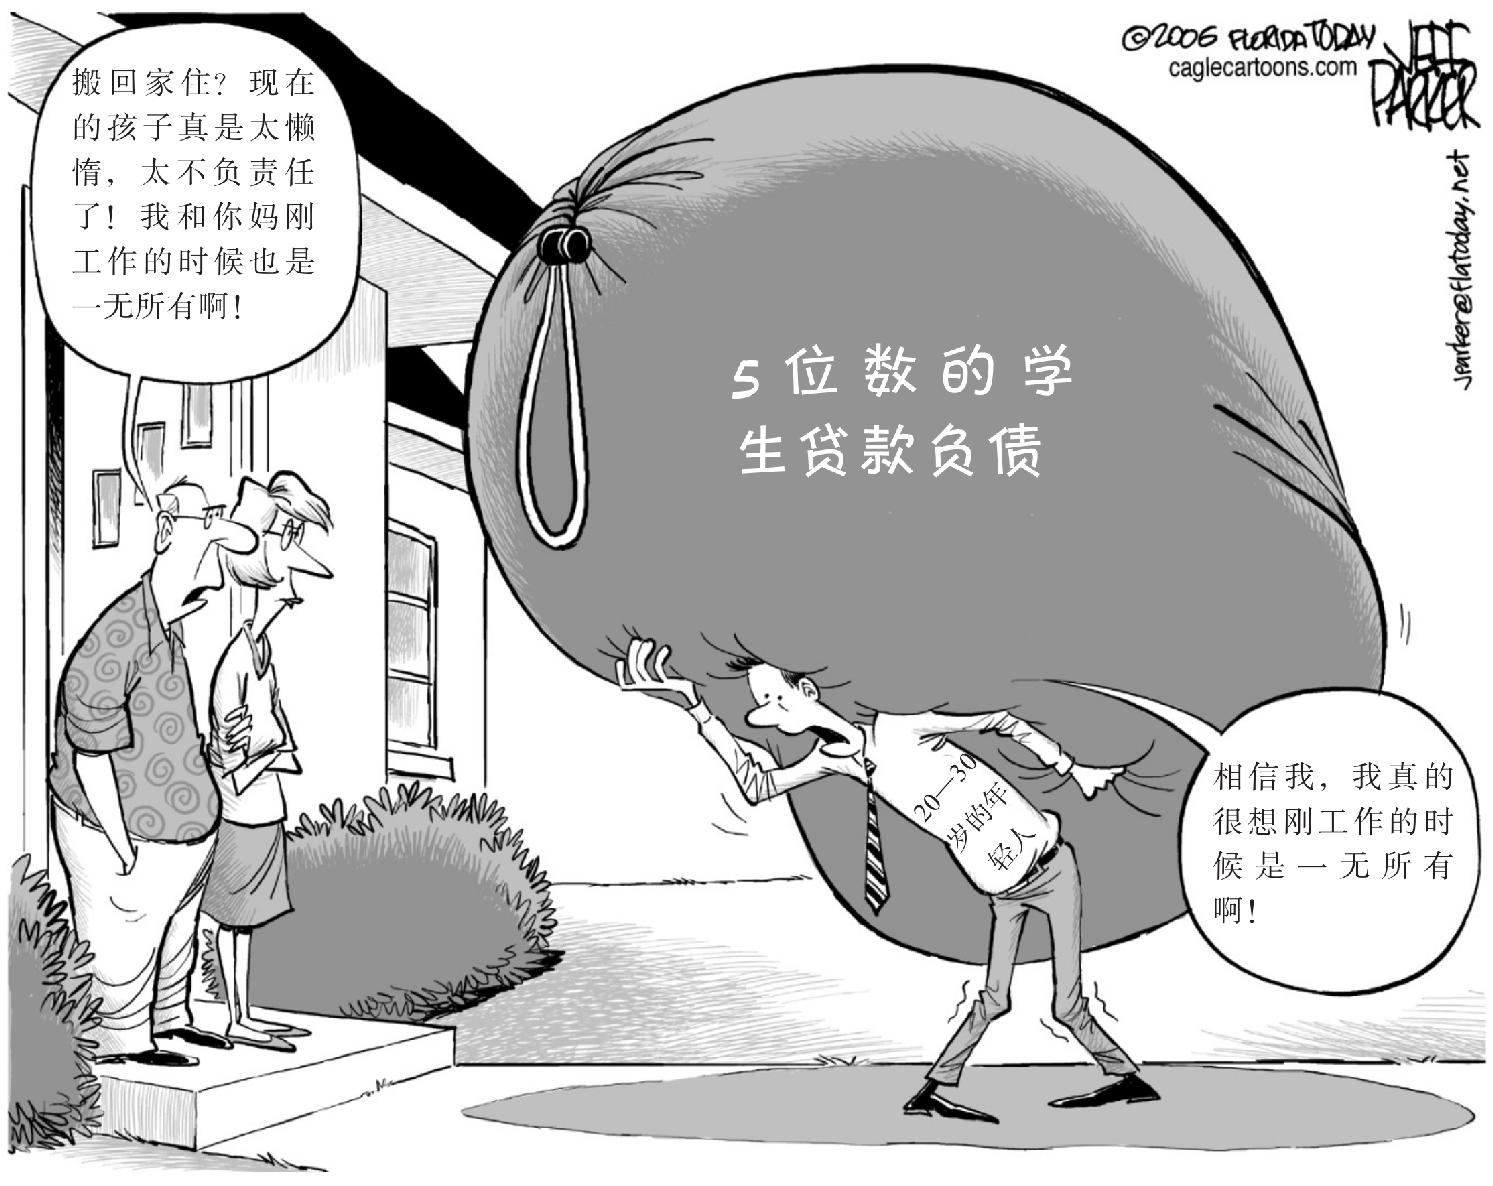
\includegraphics[width=0.80\linewidth,keepaspectratio]{image/16-1.jpg}
\caption{}\label{fig:16-1}
\end{figure}

\subsection{都工作好几年了，还在还上大学时的学生贷款}

我讲的第一个案例属于第一类人——他们年轻，欠了一大笔债。马尔科在大学毕业时，欠了一大笔学生贷款，现在他33岁了，成了一名工程师，每年能赚7.5万美元，已经相当不错了，但是他现在每年还要还2万美元的学生贷款。跟很多美国人一样，马尔科觉得他的债务在消耗他的生命——他觉得这笔学生贷款要还上一辈子了（可能真是这样，如果他选择最低还款金额，每次只还一小部分的话）。不过，马尔科预期他的薪水会持续增长，虽然比较慢，但是很稳定，预期每年增长3\%\textasciitilde{}5\%。我跟他一起制订了一个新的投资理财规划，把他收入的5\%用于偿还他的学生贷款。而且马尔科承诺以后每次加薪，都从中拿出3\%储蓄起来，放入他的自由基金。

这个新的投资理财规划给他带来什么结果呢？7年之后，他摆脱了所有债务，这感觉太棒了！除此之外，马尔科能够拿出收入的5\%做储蓄了，因为他原来要用这笔钱归还学生贷款。既然贷款还清了，他可以把原来用来还债的钱储蓄起来去投资，按照复利法则让他的自由基金不断增长。按照这个投资理财规划，马尔科再过20年就能实现财务安全了，20年听起来是一段很长的时间，但到那个时候他只有53岁。此后再过7年，也就是马尔科60岁的时候，他就能达到财务独立——比他想象的65岁退休还要早上整整5年，而且每年的退休收入比他梦想的还要多！有了这个投资理财规划后，马尔科从担心永远还不完学生贷款，转变成期待真正实现财务独立的未来幸福生活。更好的事还在后面，此后再过5年，当他65岁的时候，所有的投资增值，再加上开始领取社会保险，马尔科会实实在在地享受到他自己定义的财务自由——在制订新的投资理财规划之前，这样实现财务自由的前景对于他来说简直是想都不敢想的事情。别忘了，他制订出这个投资理财规划开始通向财务自由之旅的时候，他没有任何资产，没有任何积蓄，只有上大学欠下的债务。

\subsection{这看起来太好了，简直不像真的……但可能是真的}

接着我们来看第二类人。看了一眼他们的投资理财规划，他们马上会想，肯定哪个地方出错了。这个理财计算器肯定失灵了，他们看到自己实现财务活力或者财务独立的梦想的时间，觉得那一天来得实在太快了。“根本不可能，我实现这个财务目标简直太快了。”他们想，“我不可能这么快就实现财务独立，只要再过5年、7年、8年。这简直疯了！”在他们的脑子里，他们要实现财务独立，必须先要熬上20\textasciitilde{}30年，辛辛苦苦地工作，并且节衣缩食地生活。

哪里出现了问题呢？怎么可能这么快呢？

可能是因为他们脑子里实现财务梦想所需要的那个财富数字大得太离谱了——1000万美元，2000万美元，3000万美元。其实这根本不符合现实，只是他们凭空想出来的，他们以为自己需要很大一笔钱，才能实现财务独立，但实际并不是他们真的需要那么多钱。

凯瑟琳参加了我组织的一场财富大师研讨会，她就是一个很好的例子。凯瑟琳是一个精明能干的企业家，每年需要有10万美元的收入，才能实现财务安全——按照很多人的收入水平来看，这个目标数字太大了，但是对于她来说，这并不算大。要获得财务独立，她需要年收入17.5万美元，才能保持他现在的生活方式，而不用再去靠工作赚钱。凯瑟琳认为，自己需要超过20年的财富积累，才能达到财务独立的目标。

想不想知道，凯瑟琳和我的团队一起计算出的她实现财务梦想实际所需要的财富数字呢？结果发生了什么呢？我们发现的第一件事是，凯瑟琳的企业现在每年税后盈利超过30万美元，每年盈利增长率接近20\%。在我的团队帮助下，她又做了一些研究，然后发现她现在可以卖掉企业，价格相当于现在每年盈利的6倍，即180万美元。对于她来说，这意味着什么呢？

如果凯瑟琳卖掉自己的企业，拿到180万美元，然后用这笔钱去做投资，每年实现5\%的投资收益率，那么她每年的投资收益就有9万美元。现在她手上还有一些其他投资，每年能给她带来1万美元的投资收益。所有加在一起，凯瑟琳每年能有10万美元的投资收益。你猜到了吗？凯瑟琳现在就能实现财务安全！

凯瑟琳一听高兴坏了，但是她也很迷惑。她说：“但是托尼，现在我不想卖掉我的公司啊！”我告诉她，我并不是要鼓励她这样做，她也没有必要非得这样做。但是她完全可以宣布自己胜利了，因为她应该认识到自己现在已经实现财务安全了。为什么这么说呢？因为她现在拥有的资产，可以产生她实现财务独立所需要的收入，足够满足她现在生活的开支需要了。更加令人激动的是，按照她的企业现在每年20\%的利润增长率计算，再过3年半，她的企业价值就能增加1倍。即使他的企业盈利增长率降低一半，只有每年10\%，再过7年，企业价值也会翻倍，变成360万美元。她如果等到公司价值翻倍的时候再卖掉公司（360万美元×5\%=每年18万美元的投资收益，她什么工作都不用做），只需要3年半到7年，凯瑟琳就可以完全实现财务独立了。根本不是她原来想象的20年！而且还是在其他什么投资都不用做的情况下，凯瑟琳就能实现财务独立了！

顺便说一下，我在企业经营大师训练营上，给企业老板展示了很多经营管理上的妙招，其中有一套策略是很少有人知道的，就是让你卖掉自己企业的一部分股权（甚至是相当大的一部分股权），但是你还能继续经营、控制、指导企业，并继续从企业分享中赢利。这样做，能让你得到一大笔现金，确保你现在就能享受财务自由，同时还能继续管理你心爱的企业，让企业继续成长，享受这个过程带给你的快乐和成就感。

\subsection{你来晚了，也照样能赢}

我们再回到我的朋友安吉拉的故事。安吉拉是个普通人，从财务角度来看，她代表着美国人的平均水平。安吉拉都48岁了，过去一直过着自由自在的生活，旅行，航海，游遍全世界，她这辈子从来没有储蓄过，也没有投资过。读完本书的第一部分，她现在开始下定决心要从收入里拿出10\%储蓄起来，但是她要面对一个巨大的困难：在这场投资游戏里，她开始得太晚了。（她自己也说：“我都快50岁高龄了！”）她能利用复利巨大威力的时间不多了。

安吉拉第一次计算她要实现财务安全需要的年收入，结果算出来的数字是每年3.4万美元。要实现财务独立，她需要的年收入是5万美元。第一眼看到这个数字，她就非常激动。因为这个数字没有很多零，是她通过努力也有希望赚到的几万美元。不过，一算自己要达到这样的年收入需要多长时间，让她又从梦想回到了现实。她起步太晚了，而且每年储蓄只有收入的10\%，按照这样一个计划，安吉拉需要用上24年的时间才能实现财务安全。如果她现在才41岁，这会是一个很大的胜利，因为到65岁她就能实现财务安全了。但是因为她开始得太晚了，48岁才开始，再过24年，安吉拉就72岁高龄了。但是，要是没有这样一个规划，她会觉得自己这辈子根本不可能实现财务安全和财务独立了，有了这样一个可靠的规划，她觉得自己的未来光明多了。她非常高兴地知道，自己确实是有可能实现财务独立的。但是前面这条路非常漫长、缓慢，这确实不能让她开心、激动。

我们如何能够加快财富积累速度来更早地实现那个收入目标呢？安吉拉怎么样才能更快地实现财务安全呢？一种方法是提高收入储蓄比例，加大投资规模。她已经储蓄了收入的10\%了。考虑到她过去从来没有储蓄过，拿出收入的10\%储蓄起来，这对于她来说已经是一个很高的比例了。不过参加明天储蓄更多计划，她就能毫无痛苦地储蓄更多，因为她承诺的是以后收入提高就自动储蓄更多，这样能加快她的计划实施。加快财富积累速度的另一种方法是，承担多一点儿的风险，把投资收益率提高到7\%，甚至更多，当然，提高风险可能会带来高收益，同样也有可能带来大幅亏损。但是，结果发现，还有一个简单得多的好办法，只是我们过去一直都忽略它了。

幸运的是，安吉拉的弹药库还有一批弹药。她漏掉了一大部分未来收入，很多人也都忽略了，没有把这部分收入纳入他们的财务规划中，这一部分就是社会保险。

安吉拉已经48岁了，再有14年就年满62岁，就可以领取社会保险基金了，不过只能部分领取。再过17年，她就年满65岁，就可以全额领取了。等她年满62岁，她什么也不用干，就可以每个月领到1250美元，相当于一年1.5万美元。原来她要实现财务安全需要达到的3.4万平均年收入的目标，有了这笔收入的加入，一下子就降到1.9万美元。我们用手机App来评估这些数据，安吉拉一看，自己原来实现财务安全需要漫长的24年，有了社会保险这笔收入，现在一下子缩短了10年。也就是说，48岁的安吉拉原来要到72岁才能实现财务安全，现在有了社会保险，62岁她就能实现财务安全了。这让她激动得浑身颤抖。到那时，她不用工作，就能有足够的收入支付房贷，支付水费、电费、天然气费和电话费，支付交通费，支付基本医疗保险费。对于安吉拉来说，这真是一种自由的感觉。

不可能的事变成了可能。猜一猜，接下来又会发生什么事情？安吉拉认识到财务安全胜利在望，内心的激动和冲动激励着她。她说：“嘿，让我们再上个台阶。既然我到62岁能实现财务安全，我们来看看如何再进一步，实现财务独立，我想找到一条路，实现财务独立，不是等到我70岁甚至80岁的时候，而是60多岁就能实现财务独立！”她实现财务独立需要多少年收入呢？5万美元？只比实现财务安全需要的3.4万美元年收入多1.6万美元。

安吉拉又向前迈出了一大步。读完第三部分后，她又找到了另一种方法来加快实施她的规划。安吉拉一直对房地产投资很感兴趣，想投资一些房地产，以产生稳定的收入。她学到了一些简单的方法，投资不需要专人处理的老年人住宅，或者专为没有生活自理能力的老人提供辅助生活服务的养老住宅，通过公募或者私募房地产投资信托基金进行投资（我们会在第四部分介绍）。我们后面会讨论更多细节，但是现在可以简单地说，选择老年人住宅是投资收益性房地产的一个好方向，我称之为“人口结构不可避免的发展趋势”。7600万名婴儿潮时代出生的美国人，正在步入老年期，他们必然需要使用这些老年人住宅。每个月投资438美元，相当于每年投资5265美元，持续投资20年，假定用分配的红利再投资，继续按照复利增长，那么20年后她能积累228572美元（这里假定每年投资分红的收益率是7\%，这是现在很多老年人房地产投资信托基金的收益率水平）。

她投资养老房地产20年积累的这笔财富，以后每年会产生1.6万美元的收入（假定每年投资分红收益率为7\%），她也不用再每月追加投资来增加本金了，除非她自己想！这样的养老房地产投资还有一个巨大的好处，所有分红收入根本不用交所得税，因为资产折旧可以抵税。

马尔科、凯瑟琳、安吉拉，都是和你我一样的真实的人。你的规划就在你的能力范围之内，是你能够做到的，跟他们一样，你可以比你想象的更早地实现梦想。不要把你在应用程序上制定出来的规划1.0版本看作最终的规划。要把1.0版本看成让梦想成真之旅的起点。后面几章我会展示五种方法，让你加快财务积累的速度，更快地实现梦想。

\begin{BookQuote}
风筝飞得最高的时候，是凭借逆风，而不是顺风。

\hfill ——温斯顿·丘吉尔
\end{BookQuote}

看到财务规划所必需的目标年收入数字，再算一算达到这个收入水平所需要的持续积累财富的年数，你不管是觉得胜利并不遥远，心里非常激动，还是觉得实现梦想的路还很长，心里十分失望，都一定要振作起来——失望并不总是坏事，失望常常像是在你屁股上猛踹一脚，逼你做出巨大的改变。记住，决定我们命运的不是外部的环境，而是内心的决定。失望要么驱动我们，要么打败我们。我选择让失望驱动自己，希望你也能够采取同样的观点。大多数人做计划，甚至根本没有走到这一步，因为他们害怕发现，算出的自己实现梦想所需要积累的财富目标数字，与自己现有的财富相比差距很大，自己会感觉很失望。与其失望，不如不算，眼不见心不烦。但是你接受了挑战，承诺读完本书，走向财富自由之路。所以，你跟大多数人不一样，你选择了一条少有人走的路，而不是那条很多人走的路。

我还清清楚楚地记得那年美国国庆节的假期旅行，尽管那是20多年前的事情了。受我的好友彼得·古伯的邀请，我和一群大型电影公司的高管同行，一起穿越楠塔基特岛和马萨岛上的葡萄园。我们坐在彼得的私人游艇上，几个电影大亨正在炫耀自己的成就，如何只做了一部电影就赚了两三千万美元。我听了非常震惊——光是那个盈利的数字就让我惊呆了。我那时30多岁，当时觉得自己已经做得非常好了，绝对处于事业的上升期——我一直自我感觉非常良好，可是这次在游艇上听这群电影大亨一开口就是一年能赚几千万美元，才知道天外有天，人外有人，跟他们一比，自己赚的钱简直不值一提。这些家伙的生活方式简直太疯狂了，没过多久我就受到他们的诱惑，也想学他们那样轻松赚大钱了。

那个国庆假期的旅行经历让我很受打击，但也让我想到了一个不同的问题：我这辈子真正想要创造出什么东西呢？我有可能实现那个目标吗？那个时候我还根本没有看到，我利用自己擅长做培训的核心能力，就可以给其他人增加很大的价值，也能创造出类似水平的财务自由。

当然，拿当年的我和我当时的成就水平，跟那些电影大亨比较，对我也是不公平的。当时我才30多岁，彼得和他那些拍电影的朋友都50多岁了，有的人都快60岁了。彼得正处在事业的巅峰，我的事业才刚刚起步。他得到过5次奥斯卡金像奖提名，很多好莱坞大片上都写着他的名字。当然，那时我也小有名气了，经营着一家企业，做得也很成功——改变了自己的人生。但是我在财务上的成功，和彼得还有他那帮朋友相比，差了十万八千里。而且，我把自己和游艇上的那些家伙相比，这非常不公平，但很多人都这样做过：我痛贬自己，怪自己没能取得和那些大亨同样财富水平的成就。

但那一天，那一刻，给我带来了一个特别大的好处，就是让我置身于一个新的陌生环境里，我内心深处有个东西被改变了：我远远离开了我的舒适区。我觉得自己不属于那帮人——就像我觉得自己不配待在那里一样。你有没有过类似的感觉？这真让人吃惊，要是我们不有意识地引导大脑思考，这些想法会对我们造成多么大的影响呢！

不过，比较也是件好事。你和别人在一起，这些人玩的人生游戏比你玩的层次更高，你可能会非常沮丧，可能会非常恼火，但也可能会因此受到启发，获得灵感。那天我认识到，我并不是想要一艘游艇，但是我受到启发要好好地磨炼自己，提升自己人生游戏的比赛技能。我认识到，我可以做的，我可以给予的，我可以成就的，还有很多。对于我来说，更好的还在后头。我也意识到，在我人生的那个时点我感到非常不舒服，身处一种新的环境中，我再也不能感觉自己出众或者高人一等了，甚至远远不如别人。这样的机会逼迫我反思，对于我来说，这非常宝贵，也非常有意义。

当然，我的好友彼得邀请我到他的游艇上和他的那帮朋友一起旅行，我上面的这些想法，其实他是不知道的。他只是想召集一帮朋友，坐着他的游艇，来个国庆节快乐之旅，作为送给朋友们的一份礼物，表达他对这帮朋友的深厚友情。但是他邀请我和他的其他朋友一起旅行，给我展示了一个拥有无限可能、无限机会的世界。这次旅行的经历对我很有帮助，唤醒了我去直面真相。我很清楚地看到，自己确实有能力创造出任何我能想象得到的东西，也许我并不想拥有和他们一样的“成年人玩具”，但是我绝对可以肯定，我非常想拥有同样类型的选择，来给我的家人创造更好的生活。现在我已经50岁出头了，当年那些感觉不可能的想象，现在都变成了生活现实的平常影像。我现在过的日常生活竟然是以前的想象！但是有一点和以前一样，我还是不想要游艇。

我要说清楚，重要的不是钱，重要的是选择，重要的是自由，重要的是能够过上你想要的生活，按照你的意愿生活，而不是按照别人的意愿生活。

不要抱怨。

不要说你不能。

不要编故事骗自己。

相反，现在就做出决定！

找到上天赋予你的天赋，发挥你的天赋，服务和帮助别人，人越多越好。

如果你变得更强壮、更聪明、更有同情心、更加有能力，那么你的目标就是一个值得努力的目标。

我最早的导师之一吉姆·罗恩总是这样教导我：“你得到什么样的东西，都不会让你开心。可是你成为什么样的人，会让你非常开心或者非常伤心。”如果你每一天都能够进步，哪怕只是一点点进步，你都会为自己有所长进而感到快乐。受益于恩师的教导，我开始不断地进步，不断地思考大目标和大成就，逐渐领悟一些最重要的经验教训，其中一个最重要的经验教训是：

大多数人高估了自己一年能做成的事情，但是他们也严重低估了自己10年或者20年能够做成的事情。

事实真相是：你并不是周围环境的管理者，而是你自己生活经验的建筑师。千万不要低估长期坚持不懈地采取正确行动的威力，因为一件事不在最突出的位置，或者一件事不在你的能力范围之内。

利用复利的力量，原来看起来不可能的事情会变得可能。现在不管你是喜爱还是痛恨你的财务规划，不管你看了这个规划设定的目标会感到兴奋激动还是恐惧害怕，让我们一起把你的梦想成真计划变得更强大、更有力吧。我们要加速实现你的目标，你可以利用五大因素，让自己快马加鞭。
